\subsection{Magnetic Dipole}
Classically, the magnetic dipole is though of as a loop carrying an
electric current ($I$). 

The resultant \index{magnetic dipole moment}{magnetic dipole moment}, $\vec{\mu}$, is defined as the vector at a normal to the  
plane of the current loop, 
\begin{equation}
    \vec{\mu} = IS \vec{n}
    \label{eq:dipole_moment}
\end{equation}
where $I$ is the current in, and $S$ the surface area enclosed by, the loop. 

\begin{wrapfigure}{l}{0.4\textwidth}%
    \centering%
    % 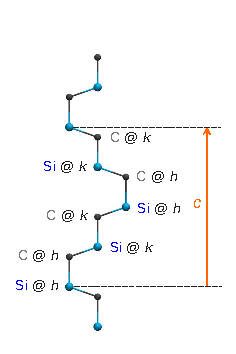
\includegraphics[width=0.38\textwidth]{figures/SiC-non-equiv-sites.pdf}%
        % B FIELD through current loop
\begin{tikzpicture}[scale=1.2, thick]
  \def\Rx{1.45}
  \def\Ry{0.43}
  \def\h{0.5}
  \def\H{3}
  \def\L{4}
  \def\NB{5}
  \def\ang{36}
  \coordinate (O) at (0,0);
  \coordinate (N) at (0,0.24*\H);
  \coordinate (M) at (0,0.45*\H);
  \coordinate (B) at (\ang:\H);
  
  % MAGNETIC FIELD
  \draw (-\Rx,0) arc (180:0:{\Rx} and {\Ry});
  \begin{scope}
    \clip ({-0.5*\L*cos(\ang)},-0.4*\H) rectangle ++({\L*cos(\ang)},\H);
    %\foreach \i [evaluate={\y=(\i-0.5)*\H/(\NB-0.5)/2;
    %                       \yl=-\H/2+(\i-0.5)*\H/(\NB-0.5)/2;}] in {1,...,\NB}{
    %  %\draw[BFieldLine,thin] (0,\y)++(\ang-180:0.5*\L) --++ (\ang:\L);
    %  %\draw[BFieldLine,thin] (0,-\y)++(\ang-180:0.5*\L) --++ (\ang:\L);
    %  \draw[BFieldLine,thin] (-\H/2,\y) -- ({-\H/2+(\H/2-\y)*cos(\ang)},\H/2);
    %  \draw[BFieldLine,thin] (-\H/2,-\y) -- ({-\H/2+(\H/2+\y)*cos(\ang)},+\H/2);
    %  \draw[BFieldLine,thin] ({\H/2-(\H/2+\yl)*cos(\ang)},-\H/2) -- (\H/2,\yl);
    %  \draw[BFieldLine,thin] ({\H/2-(\H/2-\yl)*cos(\ang)},-\H/2) -- (\H/2,-\yl);
    %}
    % \foreach \i [evaluate={\x=-0.31*\H+(\i-1)*0.62*\H/(\NB-1);
    %                        \y=-cot(\ang)*\x;
    %                        \a=0.50+0.017*\i}] in {1,...,\NB}{ %0.58-0.02*(\i-\NB/2-1)^2
    %   \draw[BFieldLine=\a] (\x,\y)++(\ang-180:\H) --++ (\ang:2*\H);
      %\fill[red] (\x,\y) circle (0.05);
    % }
  \end{scope}
  % \node[Bcol] at (\H/2,0.49*\H) {$\vb{B}$};
  
  % CIRCUIT
  \draw[white,very thick]
        (-\Rx,0) arc (-180:0:{\Rx} and {\Ry});
  \draw (-\Rx,0) arc (-180:0:{\Rx} and {\Ry});
  %\draw[white,very thick] (0,0) ellipse ({\R} and {0.3*\R});
  %\draw (0,0) ellipse ({\R} and {0.3*\R});
  %\draw (0,0) ellipse ({\R} and {0.3*\R});
  \draw[mu vector] (0,0) -- (M) node[above=-1, left=0] {$\vb*{\mu}$};
  \draw[vector] (0,0) -- (N) node[below=0,left=0] {$\vu{n}$};
  % \draw pic[->,"\small$\;\theta$",draw=black,angle radius=14,angle eccentricity=1.4]
    % {angle = B--O--N};
  \draw[white,very thick]
    (-150:{1.1*\Rx} and {1.16*\Ry}) arc (-150:-80:{1.1*\Rx} and {1.16*\Ry});
  \draw[current]
    (-135:{1.1*\Rx} and {1.16*\Ry}) arc (-135:-90:{1.1*\Rx} and {1.16*\Ry})
    node[midway,right=2,below] {$I$};
  
\end{tikzpicture}


  \caption{Schematic of current loop and induced magnetic moment.}%
\end{wrapfigure}%


The \index{magnetic dipole}{magnetic dipole} induces a magnetic field $\vec{B}$, which for points a large distance from the dipole may be calculated as \cite{Griffiths2012-pt}:
\begin{equation}
    \vec{B} = \frac{\mu_0}{4\pi} \frac{1}{r^3} \left[\frac{3(\vec{\mu} \cdot \vec{r}) \cdot \vec{r}}{r^2} - \vec{\mu}\right]
    \label{eq:}
\end{equation}

The symmetry of the field enables us to consider the direction of the dipole as aligned to the $z$-axis. Then, defining $x,y$ as usual by $r \cos\theta$ and $r \sin\theta$ respectively. We may decompose the \index{magnetic field}{magnetic field} in two separate components, parallel ($B_z$) and perpendicular ($B_x, B_y$): 
$$B_\parallel =\frac{\mu_0}{r^3}(3\cos^2 \theta - 1), \quad B_\perp = \frac{3\mu_0}{r^3}\cos\theta\sin\theta.$$
Where we use the Pythagorean principle to determine the overall magnitude $B = |\vec{B}|$ as
$$B = \sqrt{B_\parallel^2 + B_\perp^2}.$$
